\documentclass[12pt,spanish,a4paper, oneside, openany]{book}

\usepackage{graphicx}
\usepackage{setspace}	%double spacing for text, single for captions, footnotes, etc.
%\usepackage{hypernat} 	%substitut de cite que permet fer hyperlinks
% \usepackage{natbib}		% substituye a 'hypernat' que funciona en Windows.
\usepackage[square,sort,comma,numbers]{natbib}

\usepackage[utf8]{inputenc}
\usepackage[spanish]{babel}

\usepackage{lmodern} 
\usepackage{color}
\usepackage{hhline} 		% extended styles for tables
\usepackage{multirow}
\usepackage{subfigure}
\usepackage{acronym}
\usepackage{hyperref}
\usepackage{amsmath,amsmath,amssymb} 
\usepackage{fancyhdr}
\usepackage{epsfig, amsmath}
\usepackage{algorithm}
\usepackage{algorithmic}
\usepackage{pdflscape}


\selectlanguage{spanish}

% general settings
\hypersetup{
	linktocpage=true,
	colorlinks=true,
	linkcolor=blue,
	citecolor=blue,
}
\definecolor{Hgray}{gray}{0.6}

\newenvironment{definition}[1][Definition]{\begin{trivlist}
\item[\hskip \labelsep {\bfseries #1}]}{\end{trivlist}}

\setlength{\topmargin}{0cm}
\setlength{\textheight}{23cm}
\setlength{\textwidth}{17cm}
\setlength{\oddsidemargin}{0cm}
\setlength{\evensidemargin}{0cm}
\setlength{\headheight}{1cm}

\setlength{\parskip}{1em}

% indica que las 'sub-sub-sections' sean numeradas y aparezcan en el indice
\setcounter{secnumdepth}{3}
\setcounter{tocdepth}{2}

% settings for code
\renewcommand{\algorithmicrequire}{\textbf{Entrada: }}
\renewcommand{\algorithmicensure}{\textbf{Salida: }}

%%%%%%%%%%%%
% DOCUMENT %
%%%%%%%%%%%%
\begin{document}

% portada
%% portada
\newpage
\thispagestyle{empty}

\baselineskip 2em

%\vspace*{1cm}

\centerline {
\includegraphics[width=0.6\textwidth]{figs/UOC-logo}}
\begin{center}
\textsc{Universitat Oberta de Catalunya (UOC) \\
 Máster Universitario en Ciencia de Datos (\textit{Data Science})\\}

%\centerline {\pic{UOC}{4cm}}

\vspace*{1.5cm}

\textsc{\Large TRABAJO FINAL DE MÁSTER}


%\textbf{\Huge VirtualTechLab Model: }

\vspace*{1.5cm}

\textbf{\Large Aplicación de algoritmos de aprendizaje automático para predecir disfunción cognitiva en pacientes de esclerosis múltiple mediante índices de conectividad estructural}

%% \textbf{\large xxx subtítulo (en caso de existir) xxx}

\vspace{2.5cm}
\baselineskip 1em

\vspace{1cm}
\baselineskip 2em
-----------------------------------------------------------------------------\\
Autor:      Efraín Lima Miranda\\
Tutor:   Dr. Eloy Martínez de las Heras\\
Co-Tutor:   Dra. Sara Llufriu\\
Profesor: Dr. Jordi Casas Roma\\

-----------------------------------------------------------------------------\\
\vspace*{1.5cm}
Barcelona, \today

\end{center}



\newpage
\pagestyle{empty}
\hfill

%% copyright

\includegraphics[width=0.3\textwidth]{figs/previos/copyright.png}

Copyright © 2018 Efraín Lima Miranda

Esta obra está sujeta a una licencia de Reconocimiento-NoComercial-CompartirIgual 3.0

España de CreativeCommons (CC BY-NC-SA 3.0 ES) 

\url{http://creativecommons.org/licenses/by-nc-sa/3.0/es/}

\newpage

% ficha
\begin{center}

\textbf{FICHA DEL TRABAJO FINAL}

% Please add the following required packages to your document preamble:
% \usepackage{multirow}
\begin{table}[H]
\centering
\label{my-label}
\begin{tabular}{|r|l|}
\hline
\multirow{3}{*}{\textbf{Título del trabajo:}}          & Aplicación de algoritmos de aprendizaje automático   \\
                                                       & para predecir disfunción cognitiva en pacientes de   \\ 
                                                       & esclerosis múltiple mediante índices de conectividad \\
                                                       & estructural \\            
\hline
\textbf{Nombre del autor:}                             & Efraín Lima Miranda                                \\
\hline
\textbf{Nombre de los} & Dr. Eloy Martínez de las Heras                   \\ 
\textbf{colaboradores}  & Dra. Sara Llufriu                                 \\
                                                       \hline
\textbf{Nombre del PRA:}                               & Dr. Jordi Casas Roma                               \\ 
\hline
\textbf{Fecha de entrega:}                              & Junio de 2018 \\ 
\hline

\textbf{Titulación o programa:}                        & Máster Universitario en Ciencia de Datos (\textit{Data Science}) \\
\hline
\textbf{Área del Trabajo Final:}                       & Aprendizaje automático                                 \\ 
\hline
\textbf{Idioma:}                       & Español                                 \\ 

\hline
\textbf{Palabras clave:}                               & aprendizaje automático, conectividad estructural, \\
                                                       & esclerosis múltiple, rendimiento cognitivo \\ 
\hline

\end{tabular}
\end{table}

\null\vfill

\end{center}
\newpage


% dedicatoria
\thispagestyle{empty}

\parbox{0.6\textwidth}{\hspace{0.6\textwidth}}
\parbox{0.4\textwidth}{\bigskip\bigskip\bigskip\bigskip\bigskip\bigskip\bigskip\textit{ 
Dedicado a Laura, mi felicidad de cada día.
}}
\hfill
\newpage

% dedicatoria
\thispagestyle{empty}

\noindent
\textbf{\begin{Large}\textit{Agradecimientos}\end{Large}}
\newline
\newline
\noindent\textit{
Deseo expresar mi más sincero agradecimiento al tutor de este proyecto Dr. Eloy Martínez de las Heras por
sus apoyo personal y humano durante todo este trabajo.\\

A sí mismo, a todo el equipo del XXXX por su trabajo previo}

% resumen
\chapter*{Resumen}
\addcontentsline{toc}{chapter}{Resumen}
\onehalfspacing

\pagenumbering{roman} 
\setcounter{page}{1} 
\pagestyle{plain}
Este trabajo tiene como objetivo la predicción del rendimiento cognitivo del paciente con esclerosis múltiple (EM) a través de la cuantificación del volumen lesional y la microestructura de la red cerebral empleando herramientas de aprendizaje automático. Esta enfermedad neurodegenerativa es una de las causas más importantes de discapacidad física y cognitiva en adultos jóvenes.

Para esta investigación se ha dispuesto de una muestra de 182 sujetos, donde 140 padecen de EM y 42 son controles sanos. De cada uno de ellos se dispone de cuatro medidas de tensor de difusión (DTI) (Anisotropía fraccional, Difusividad media, Difusividad axial y Difusividad radial), número de fibras y volumen lesional. Toda esta información proveniente del análisis de la conectividad estructural  es presentada mediante matrices simétricas.

Tras realizar las tareas de preprocesamiento y limpieza de toda esta información, con el software NeuLoadData, se han estimado los mejores parámetros de configuración para los algoritmos ``Logistic Regression'', ``Support Vector Machine (SVM)'', ``Gaussian Naive Bayes, Random Forest Classifier'' y ``Artificial Neural Network (ANN)''. Usando únicamente las medidas de tensor de difusión todos los modelos obtenidos han sido capaces de predecir exitosamente más del 75\%. Por lo tanto, el enfoque propuesto de aprendizaje automático para la predicción el rendimiento cognitivo en pacientes con EM ha demostrado su utilidad e interés como herramienta para analizar un gran conjunto de datos satisfactoriamente en el campo sanitario.

\vspace*{1cm}

\textbf{Palabras clave:} aprendizaje automático, conectividad estructural, esclerosis múltiple, rendimiento cognitivo

% abstract
%\chapter*{Abstract}
%\addcontentsline{toc}{chapter}{Abstract}
%\onehalfspacing
%\vspace*{1cm}
The present study aims to predict the cognitive performance of patients with multiple sclerosis (MS) through quantification of lesional volume and the microstructure of the brain network by means of machine learning techniques. This neurodegenerative disease is one of the main causes of both physical and cognitive disability in young adults.

For this research, we have a sample of 140 patients with Multiple Sclerosis and 42 healthy controls. For each participant, information relating to four measures of diffusion tensor (DTI) (fractional anisotropy, medium diffusivity, axial diffusivity and radial diffusivity), number of fibers and lesional volume has been recorded. All this information coming from the analysis of structural connectivity is presented by symmetric matrices.

After carrying out preprocessing tasks on all of this information using the NeuLoadData software, the best configuration parameters have been estimated for the algorithms Logistic Regression, Support Vector Machine (SVM), Gaussian Naive Bayes, Random Forest Classifier and Artificial Neural Network (ANN). Making use of only diffusion tensor measurements, all the models have had a successful prediction rate of over 75\%. Therefore, the proposed approach of machine learning for prediction cognitive performance in patients with MS has demonstrated satisfactorily its usefulness and interest as a tool to analyze a large set of data in the health field.

\textbf{Keywords:} manchine learning, structural connectivity, multiple sclerosis, cognitive performance


\pagestyle{fancy}
\renewcommand{\chaptermark}[1]{ \markboth{#1}{}}
\renewcommand{\sectionmark}[1]{\markright{ \thesection.\ #1}}
\lhead[\fancyplain{}{\bfseries\thepage}]{\fancyplain{}{\bfseries\rightmark}}
\rhead[\fancyplain{}{\bfseries\leftmark}]{\fancyplain{}{\bfseries\thepage}}
\cfoot{}

% indice
\cleardoublepage
\phantomsection
\addcontentsline{toc}{chapter}{Índice}
\tableofcontents

% listado de figuras
\cleardoublepage
\phantomsection
\addcontentsline{toc}{chapter}{Listado de Figuras}
\listoffigures

% listado de tablas
\cleardoublepage
\phantomsection
\addcontentsline{toc}{chapter}{Listado de Tablas}
\listoftables

\thispagestyle{empty}

\pagenumbering{arabic}

\pagestyle{fancy}
\renewcommand{\chaptermark}[1]{ \markboth{#1}{}}
\renewcommand{\sectionmark}[1]{\markright{ \thesection.\ #1}}
\lhead[\fancyplain{}{\bfseries\thepage}]{\fancyplain{}{\bfseries\rightmark}}
\rhead[\fancyplain{}{\bfseries\leftmark}]{\fancyplain{}{\bfseries\thepage}}
\cfoot{}

\onehalfspacing

% PROLEGÓMENO
\part{Prolegómeno}
\null\vfill
\chapter{Introducción}
\label{chapter:introduccion}

La \gls{em} es una enfermedad neurodegenerativa crónica, inflamatoria y desmielinizante del \gls{snc}, de carácter autoinmune y considerada como una de las causas más importantes de discapacidad física y cognitiva en adultos jóvenes \cite{Rocca2015ClinicalSclerosis}. Esta enfermedad se caracteriza principalmente por la presencia de placas desmielinizadas focales, y por una afectación microestructural difusa más allá de las lesiones en la gls{sban} y la \gls{sgan}. Ambos componentes son los responsables de la atrofia cerebral y, en cierta medida, están asociados con la discapacidad cognitiva \cite{Kutzelnigg2014PathologyDiseases}. Este deterioro cognitivo está presente en el 40-70\% de los pacientes, incluso durante etapas tempranas de la enfermedad. Los déficits cognitivos más comunes son los relacionados con la atención, las funciones ejecutivas, la velocidad de procesamiento de la información y la memoria episódica \cite{Chiaravalloti2008CognitiveSclerosisb}. 

La \gls{rm} convencional ha demostrado ser una  técnica útil para el diagnóstico y monitorización de la enfermedad de \gls{em}.  La presentación de lesiones características de la enfermedad se muestran hipointensas en secuencias potenciadas en T1 y con un aumento de señal en secuencias potenciadas en T2. Sin embargo, la presencia de lesiones y las manifestaciones clínicas de los pacientes son modestas \cite{Barkhof2002TheRevisited}. Probablemente, a causa de la baja especificidad en la patología subyacente y a la baja sensibilidad del daño del tejido de apariencia normal en este tipo de secuencias.  La existencia de nuevas modalidades de imagen por RM, denominadas \gls{rm} avanzada o no convencional, ha aportado información más sensible más allá de las lesiones focales, permitiendo estudiar el tejido de apariencia normal, siendo una de las modalidades más populares actualmente es la \gls{drm}. Esta técnica de \gls{rm} se basa en el estudio del movimiento de las moléculas de agua y permite caracterizar las trayectorias de \gls{sb} de forma no invasiva, dado que en la \gls{sb} este movimiento de moléculas de agua predomina en la dirección paralela al axón y se encuentra limitado en su dirección perpendicular \cite{Basser2000InDatab}.  Por tanto, a partir de la \gls{drm} podemos obtener datos cuantitativos y patológicamente más específicos capaces de detectar cambios en la integridad microestructural en \gls{sban} y \gls{sgan}. A partir de la \gls{drm} podemos obtener unas medidas que se conocen como \gls{dti}. Estas medidas cuantifican la direccionalidad y magnitud del movimiento de las moléculas de agua en el espacio tridimensional. Dado que existe una fuerte direccionalidad debido a la presencia de mielina y axones en la \gls{sb}, el movimiento es anisotrópico y puede representarse como una elipsoide, donde el semieje principal indica la máxima difusividad. La elipsoide se puede parametrizar por un conjunto de vectores y valores propios que nos proporcionan unos índices sensibles a la integridad del tejido. El más común es la \gls{fa}. La \gls{fa} es una variable numérica cuyos valores oscilan entre 0 (máxima isotropía) y 1 (máxima anisotropía). La \gls{fa} es mayor en la \gls{sb} que en la \gls{sg}, debido a que la movilidad del agua está altamente influenciada por la organización de las fibras nerviosas. Por este motivo, el valor de \gls{fa} es comúnmente utilizado en los estudios como un marcador de la integridad estructural, ya que la pérdida de barreras reduce el grado de anisotropía (menor \gls{fa}). Hay otros valores del tensor que se pueden cuantificar como: la \gls{md}, la \gls{ad} y la \gls{rd}. Mientras que la \gls{fa} y la \gls{md} se han asociado a diversos cambios patológicos en el tejido, los cambios de \gls{ad} y \gls{rd} se han asociado con daño axonal y desmielinización principalmente en estudios con modelos animales \cite{Song2005DemyelinationBrain}.

Mediante el tensor de difusión es posible generar una representación de las fibras de la \gls{sb} o tractografía. La tractografía utiliza la dirección de máxima difusividad entre vóxeles cercanos para trazar las diferentes conexiones que componen la red cerebral. Sin embargo, esta aproximación es muy simplista dado que el modelo por \gls{dti} no es capaz de descomponer las diferentes fibras contenidas en un solo vóxel. La estructura local de la SB presenta regiones de cruce, dobleces o dispersión de fibras en más del 90\% de los vóxeles \cite{Jeurissen2013InvestigatingImaging}, El uso de modelos avanzados de tractografía proporciona una representación de mayor resolución angular de los diferentes máximos locales contenidos dentro del vóxel y reemplaza la representación de la elipsoide por otra estimación más compleja \cite{Tuch2002HighHeterogeneity}. Gracias a esto se puede descomponer las fibras de \gls{sb} en diferentes direcciones en una región de cruce de fibras y reconstruir aquellos tractos que presentan una gran curvatura y una baja \gls{fa} \cite{Martinez-Heras2015ImprovedRadiation}.  

La realización de la modelos avanzados de tractografía permite generar fibras de \gls{sb} biológicamente más precisas respecto a la anatomía subyacente y trazar las trayectorias que componen la red cerebral \cite{Rubinov2010ComplexInterpretations}. Una vez generada la  tractografía es posible cuantificar la reconstrucción con diferentes índices como pueden ser el número de fibras, el volumen lesional de las conexiones o las medidas del tensor. Esto puede facilitar el uso de medidas sensibles para diferenciar entre un cerebro sano y otro con presencia de una patología. Además de la posibilidad de detectar qué conexiones del cerebro (subsistemas) guardan algún tipo de relación con variables clínicas de interés \cite{Llufriu2017StructuralSclerosis}. 

A través de la cuantificación de este tipo de medidas sensibles a la microestructura tisular se pueden relacionar cambios patológicos de la \gls{sban} con el deterioro cognitivo en pacientes con \gls{em} \cite{Gabilondo2014Trans-synapticSclerosis} \cite{Llufriu2017StructuralSclerosis}. Otra herramienta útil para la detección de anomalías de la red cerebral es la teoría de grafos \cite{Bullmore2009ComplexSystems}. Esta metodología permite caracterizar varios aspectos de la estructura de la red, designando las distintas regiones de interés (\gls{sg}) como nodos de un grafo y las conexiones entre estos nodos como aristas (\gls{sb}). Este planteamiento ha facilitado la comprensión de la arquitectura de la red cerebral. Basándose en estos métodos, estudios recientes han demostrado que el cerebro no puede ser considerado simplemente como una gran red interconectada, sino más bien una colección jerárquica de redes de ámbito local que cooperan paralelamente y son capaces de optimizar información por medio de diferentes estructuras modulares \cite{Sporns2011NetworksBrain}. 

El uso de herramientas de análisis de la conectividad estructural en los pacientes con \gls{em} ha demostrado que la red cerebral de estos pacientes tienen una menor capacidad para intercambiar y procesar información eficazmente. Además, la existencia de mecanismos de desconexión ha sido descrita como una causa importante en la manifestación de la alteración cognitiva en la \gls{em} \cite{Shu2011DiffusionSclerosis} \cite{Llufriu2017StructuralSclerosis} \cite{Bozzali2013AnatomicalSclerosis} \cite{Louapre2014BrainStudy} \cite{Dineen2009DisconnectionSclerosis}. Sin embargo, a pesar de estos importantes hallazgos, hay que tener en cuenta otros factores que pueden relacionarse con el rendimiento cognitivo como el volumen lesional y el daño tisular local de la \gls{sb} \cite{Stellmann2017ReducedMS} \cite{Ouellette2018LesionSclerosis.}. 

Como herramienta de análisis de este trabajo se introduce el aprendizaje automático para el estudio de la conectividad estructural de los pacientes con \gls{em}. El aprendizaje automático forma parte de las ciencias computacionales caracterizándose por la búsqueda de modelos capaces de generalizar comportamientos implícitos en los datos haciendo que "aprendan" automáticamente a partir de la información proporcionada. La tarea de clasificación es una de las más importantes entre todo el conjunto de algoritmos que se engloban en las técnicas de aprendizaje automático. Utilizando algoritmos supervisados, se caracteriza por la búsqueda de un modelo capaz de asignar un conjunto de clases, o etiquetas, basándose en la información contenida en los datos. Estas técnicas de aprendizaje automático han ayudado a numerosos estudios a obtener resultados muy positivos, como por ejemplo, a la hora de diferenciar entre pacientes con \gls{em} y sujetos sanos basándose en la información contenida en las imágenes de \gls{rm} \cite{Zhang2016ComparisonMachine}.





% capítulos del documento
Una vez que obtenemos para cada algoritmos la mejor combinación de resultados, se ejecutan los modelos calculados con el conjunto de test y de entrenamiento inicial. De esta forma se pretende estimar el sobreajuste, ``overfitting'', del modelo. 

\section{Concepto de sobreajuste}
\label{section:sobreajuste}
El sobreajuste u ``overfitting'' se produce cuando un modelo cuando obtiene muy buenos resultados bien con los datos de entrenamiento, pero su precisión es notablemente más baja con el conjunto de test. Esto se produce porque el modelo se ha adaptado a los valores del conjunto de entrenamiento y no es capaz de generalizar para datos que no ha procesado. En la imagen \ref{figure:sobreajuste} podemos observar gráficamente en que consiste este problema.

\begin{figure}[H]
\centering
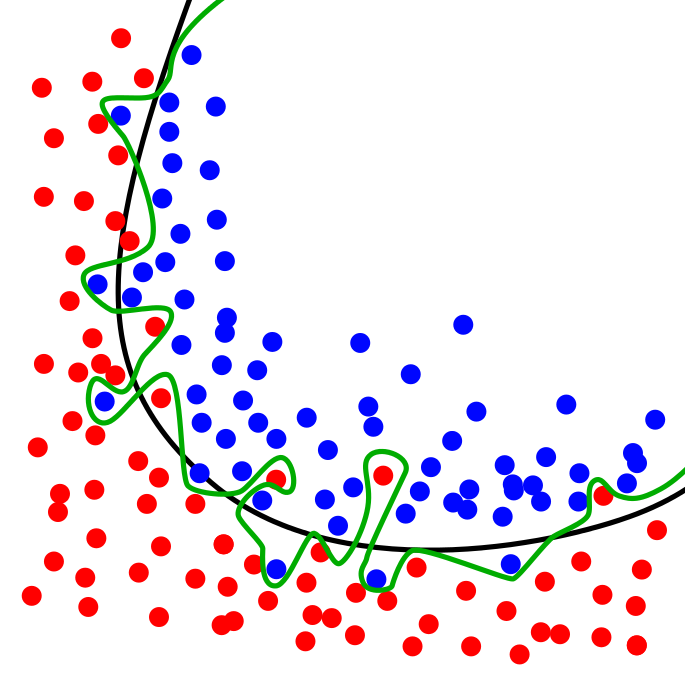
\includegraphics[width=0.3\textwidth]{figs/Overfitting.png}
\caption{Ejemplo de sobreajuste, línea verde \cite{SobreajusteLibre}}
\label{figure:sobreajuste}
\end{figure}

Este sobreajuste está directamente relacionado con la complejidad del modelo, cuanto más complejo sea más tendencia tendrá a sobreajustarse. Aparte, si el conjunto de datos del que disponemos es reducido, como en nuestro caso, este problema de sobreajuste estará muy presente.

\section{Resumen de los resultados}

En la tabla \ref{table:resultados} podemos ver para cada algoritmo los resultados obtenidos cuando se ejecuta la mejor configuración obtenida en los pasos anteriores. Entre los resultados se distinguen los valores para el conjunto de entrenamiento y para el conjunto de test. De esta forma controlamos el sobreajuste anteriormente descrito.


\begin{table}[H]
\centering
\begin{tabular}{c|c|c|c|c|}
\cline{2-5}
                                        & \multicolumn{2}{c|}{\textbf{Todas las matrices}} & \multicolumn{2}{c|}{\textbf{Matrices de DTI}} \\ \cline{2-5} 
                                        & \textbf{Test}          & \textbf{Train}          & \textbf{Test}         & \textbf{Train}        \\ \hline
\multicolumn{1}{|c|}{\textbf{Logistic Regression}} & 72.73\%                & 67.69\%                 & 78.57\%               & 84.42\%               \\ \hline
\multicolumn{1}{|c|}{\textbf{Support Vector Machine}}      & 72.73\%                & 100\%                   & 78.72\%               & 100\%                 \\ \hline
\multicolumn{1}{|c|}{\textbf{Gaussian Naive Bayes}}    & 60.61\%                & 70.77\%                 & 78.72\%               & 86.02\%               \\ \hline
\multicolumn{1}{|c|}{\textbf{Random Forest Classifier}}   & 72.73\%                & 96.92\%                 & 74.47                 & 93.55\%               \\ \hline
\multicolumn{1}{|c|}{\textbf{Artificial Neural Network}}      & 65.00\%                & 70.51\%                 & 82.14                 & 82.14\%               \\ \hline
\end{tabular}
\caption{Tabla resumen de los resultados de los experimentos por algoritmo}
\label{table:resultados}

\end{table}

\section{Precisión,  exhaustividad y  medida-F1}

En las imágenes 
\ref{figure:logall}, 
\ref{figure:logdti}, 
\ref{figure:svmall}, 
\ref{figure:svmdti}, 
\ref{figure:bayesall}, 
\ref{figure:bayesdti},
\ref{figure:forestall},
\ref{figure:forestdit},
\ref{figure:annall} y
\ref{figure:anndti},
 extraídas de los resultados podemos ver para cada algorimos los resultados de las dos ejecuciones: considerando todas las matrices o solamente las \gls{dti}. En cada una se puede ver para cada clase (1, 0) los valores de precisión (precision), exhaustividad (recall) y la medida-F1 (f1-score) para cada uno de las ejecuciones. Estas tres medidas están relacionadas con los errores de tipo I y tipo II. 

\begin{figure}[H]
\centering
\fbox{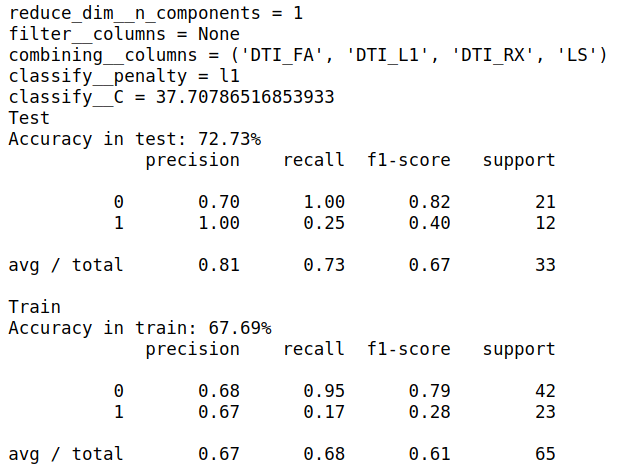
\includegraphics[width=0.5\textwidth]{figs/resultados/log_all.png}}
\caption{Resultado ejecución algoritmo Logistic Regression. Considerando todas las matrices.}
\label{figure:logall}
\end{figure}

\begin{figure}[H]
\centering
\fbox{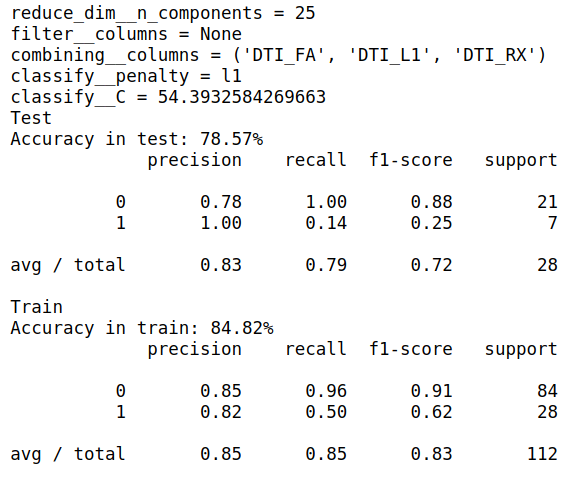
\includegraphics[width=0.5\textwidth]{figs/resultados/log_dti.png}}
\caption{Resultado ejecución algoritmo Logistic Regression. Considerando sólo matrices \gls{dti}.}
\label{figure:logdti}
\end{figure}

\begin{figure}[H]
\centering
\fbox{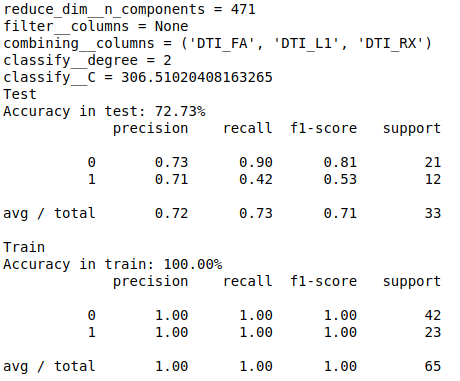
\includegraphics[width=0.5\textwidth]{figs/resultados/svm_all.png}}
\caption{Resultado ejecución algoritmo Support Vector Machine. Considerando todas las matrices.}
\label{figure:svmall}
\end{figure}

\begin{figure}[H]
\centering
\fbox{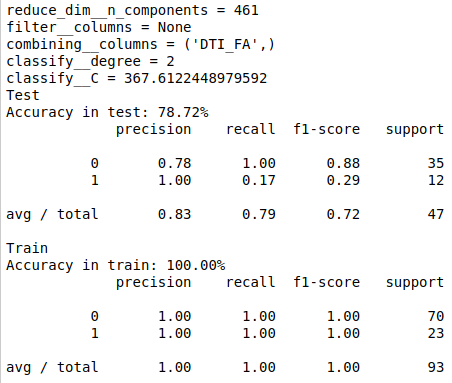
\includegraphics[width=0.5\textwidth]{figs/resultados/svm_dti.png}}
\caption{Resultado ejecución algoritmo Support Vector Machine. Considerando sólo matrices \gls{dti}.}
\label{figure:svmdti}
\end{figure}

\begin{figure}[H]
\centering
\fbox{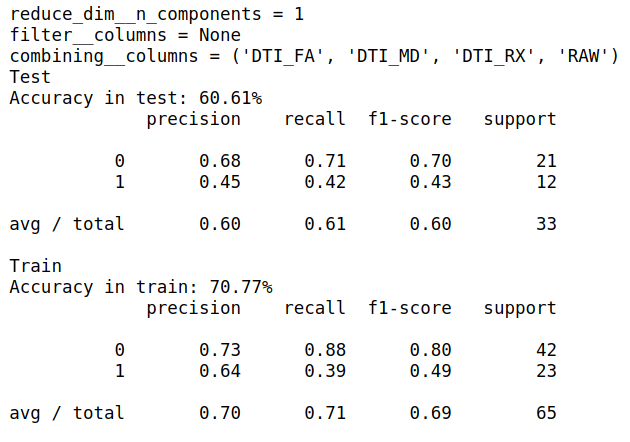
\includegraphics[width=0.5\textwidth]{figs/resultados/bayes_all.png}}
\caption{Resultado ejecución algoritmo Gaussian Naive Bayes. Considerando todas las matrices.}
\label{figure:bayesall}
\end{figure}

\begin{figure}[H]
\centering
\fbox{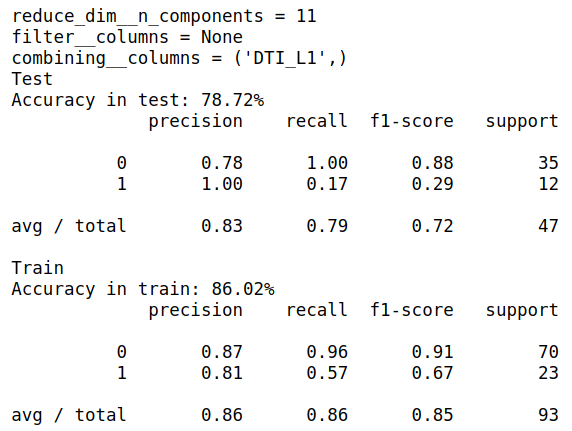
\includegraphics[width=0.5\textwidth]{figs/resultados/bayes_dti.png}}
\caption{Resultado ejecución algoritmo Gaussian Naive Bayes. Considerando sólo matrices \gls{dti}.}
\label{figure:bayesdti}
\end{figure}

\begin{figure}[H]
\centering
\fbox{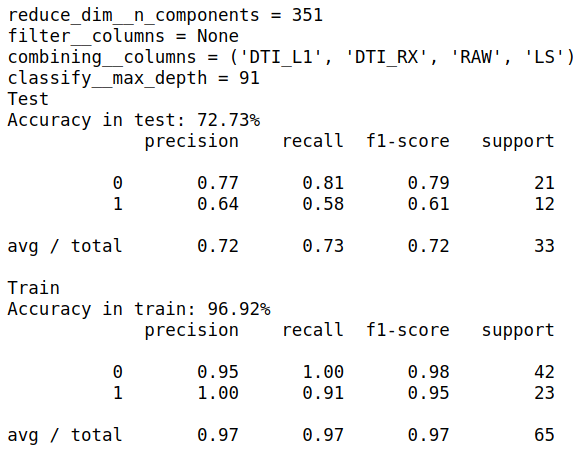
\includegraphics[width=0.5\textwidth]{figs/resultados/forest_all.png}}
\caption{Resultado ejecución algoritmo Random Forest Classifier. Considerando todas las matrices.}
\label{figure:forestall}
\end{figure}

\begin{figure}[H]
\centering
\fbox{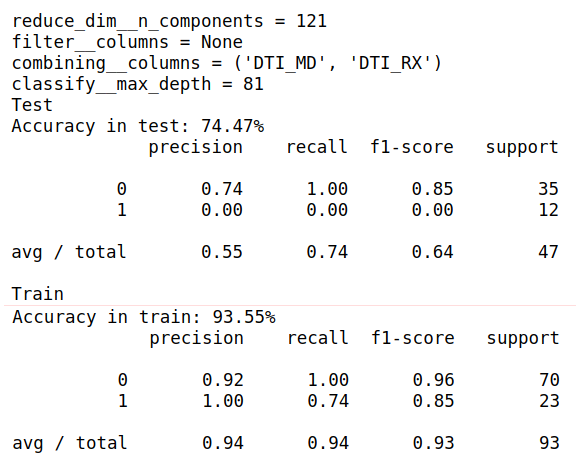
\includegraphics[width=0.5\textwidth]{figs/resultados/forest_dti.png}}
\caption{Resultado ejecución algoritmo Random Forest Classifier. Considerando sólo matrices \gls{dti}.}
\label{figure:forestdit}

\end{figure}
\begin{figure}[H]
\centering
\fbox{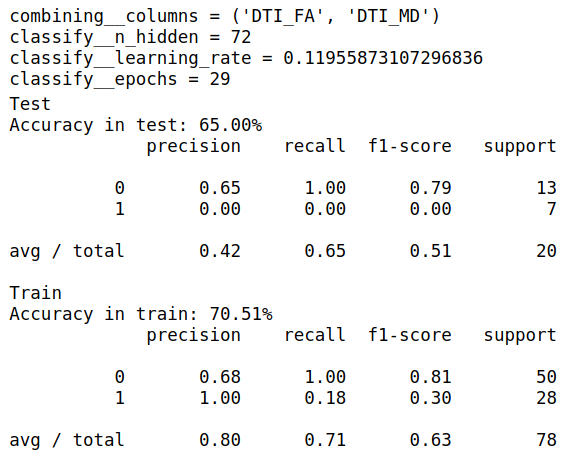
\includegraphics[width=0.5\textwidth]{figs/resultados/ann_all.png}}
\caption{Resultado ejecución algoritmo Artificial Neural Network. Considerando todas las matrices.}
\label{figure:annall}
\end{figure}

\begin{figure}[H]
\centering
\fbox{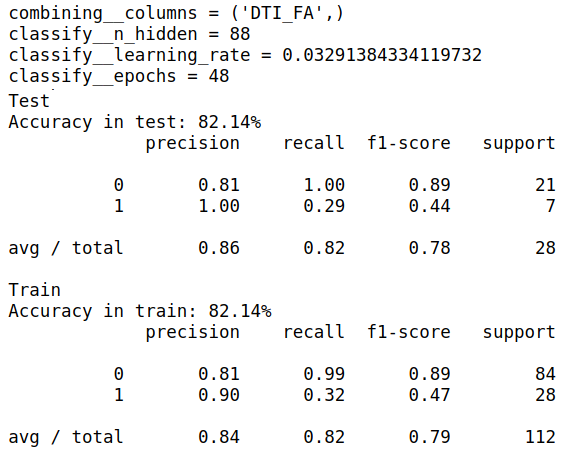
\includegraphics[width=0.5\textwidth]{figs/resultados/ann_dti.png}}
\caption{Resultado ejecución algoritmo Artificial Neural Network. Considerando sólo matrices \gls{dti}.}
\label{figure:anndti}
\end{figure}

La precisión es la habilidad del clasificador etiquetar correctamente los valores dentro de su grupo. La exhaustividad en cambio es la habilidad para acertar con las etiquetas en todo el conjunto. Por ejemplo, si disponemos de 10 ejemplares de donde 3 son del tipo A y 7 son del tipo B. A través de nuestro modelo obtenemos 5 elementos del tipo A pero sólo 2 han sido correctamente etiquetados, entonces nuestra precisión sería 2/3 y la exhaustividad 2/10. La medida-F1 engloba las otras dos siendo un valor único ponderado de la precisión y la exhaustividad. Su valor se calcula con la siguiente fórmula: 

$$F_1 = \frac{2}{\tfrac{1}{\mathrm{recall}} + \tfrac{1}{\mathrm{precision}}} = 2 \cdot \frac{\mathrm{precision} \cdot \mathrm{recall}}{\mathrm{precision} + \mathrm{recall}}$$

Aunque en este trabajo nos hemos centrado en una mejor ``accuracy'' pero igualmente, dependiendo de la finalidad de los experimentos se pueden ajustar para que la selección de los parámetros de la configuración tuviese como meta alguno de éstos.



% bibliografía
\addcontentsline{toc}{chapter}{Bibliografía}
\bibliographystyle{alphadin} % IEEEtran or alphadin??

\bibliography{mendeley_v2}

\end{document}